\twocolumn[\colorsection{Ley de Gauss}]
\setcounter{figure}{0}

\begin{Exercise}\label{p:gauss01}
	En la figura \ref{f:gauss01} se muestra una región del espacio donde existe un campo eléctrico uniforme de módulo $|\va*{E}| = \SI{2.5E5}{\newton/\coulomb}$, formando un ángulo de $30^\circ$ respecto del plano $ij$. Calcular el flujo de este campo eléctrico a través de la superficie circular mostrada en la figura, paralela al plano $ij$ y de radio igual a $\SI{5}{\centi\metre}$.
\end{Exercise}
\begin{Answer}
	$\SI{980}{\newton . \metre\squared/\coulomb}$
\end{Answer}
%
\begin{minipage}[t]{.5\textwidth}
	\begin{center}
	\tdplotsetmaincoords{70}{110}
	\begin{tikzpicture}[tdplot_main_coords, scale=0.5]
		%Axis
		\filldraw[fill=green, opacity=0.2,tdplot_main_coords] (4,0,0) arc (0:360:4);

		\draw[blue, dotted,-{latex}] (0,0,0) -- (6,0,0) node [pos=1.1] {$i$};
		\draw[blue, dotted,-{latex}] (0,0,0) -- (0,6,0) node [pos=1.05] {$j$};
		\draw[blue, dotted,-{latex}] (0,0,0) -- (0,0,4)  node [left] {$k$};

		\foreach \y in {-3,0,3}{
			% \foreach \r in {-6,-3,...,6}{
			\foreach \r in {-3,0,3}{
				\draw[-{latex}] (\r,\y,0) -- (\r,\y+1.73,1);
				\draw[] (\r,\y+1.73,1) -- (\r,\y+3.46,2);
			}
		}

		\draw[] (-3,-3-0.2*1.73,-0.2*1) -- (-3,-3,0);
		\draw[] (-3,3-0.1*1.73,-0.1*1) -- (-3,3,0);
		\draw[] (3,-1.73,-1) -- (3,-0.39*1.73,-0.39*1);
		\draw[] (0,-3-1.73,-1) -- (0,-3-0.7*1.73,-0.7*1);
		\draw[] (3,-3-1.73,-1) -- (3,-3,0) node [above,pos=0.2] {$\va*{E}$};
		\draw[] (3,3-1.73,-1) -- (3,3,0);
	\end{tikzpicture}
	\captionof{figure}{Problema \ref{p:gauss01}\label{f:gauss01}}
	\end{center}
\end{minipage}
\begin{minipage}[t]{.5\textwidth}
	% \strut\vspace*{-\baselineskip}
	\begin{center}
		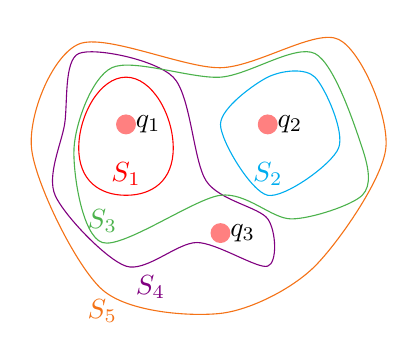
\begin{tikzpicture}[scale=0.6]
			\draw [red] plot [smooth cycle, tension=1] coordinates {(0,0) (1,1.5) (2,0) (1,-1)} node [above] {$S_1$};

			\draw [violet] plot [smooth cycle, tension=0.5] coordinates {(-0.5,-1) (-0.3,.5) (0,2) (2,1.5) (2.7,-0.7) (4,-1.5) (4,-2.5) (2.5,-2) (1,-2.5)} node [below right] {$S_4$};

			\draw [cyan, xshift=3cm] plot [smooth cycle, tension=0.5] coordinates {(0,0.5) (1,1.5) (2,1.5) (2.5,0) (1,-1)} node [above] {$S_2$};

			\draw [green!40!gray] plot [smooth cycle, tension=0.5] coordinates {(-0.1,0) (0.7,1.7) (3,1.5) (5,2) (6,0) (6,-1) (4.5,-1.5) (3,-1)  (0.5,-2)} node [above] {$S_3$};

			\draw [yellow!40!red] plot [smooth cycle, tension=0.5] coordinates {(-1,0) (0,2.2) (3,1.7) (5.5,2.3) (6.5,0) (5,-2.5) (3,-3.5)  (0.5,-3)} node [below] {$S_5$};
			\fill [red!50](1,0.5) circle(6pt) node[black, right] {$q_1$};
			\fill [red!50](4,0.5) circle(6pt) node[black, right] {$q_2$};
			\fill [red!50](3,-1.8) circle(6pt) node[black, right] {$q_3$};
		\end{tikzpicture}
		\captionof{figure}{Problema \ref{p:gauss02}\label{f:gauss02}}
	\end{center}
\end{minipage}
%
\begin{Exercise}\label{p:gauss02}
	Las tres esferas pequeñas que se ilustran en la figura \ref{f:gauss02} tienen cargas $q_1 = \SI{4.0}{\nano\coulomb}$, $q_2 = \SI{-7.8}{\nano\coulomb}$ y $q_3 = \SI{2.4}{\nano\coulomb}$. Calcular el flujo eléctrico neto a través de cada una de las siguientes superficies cerradas que se ilustran en sección transversal en la figura: \textit{a}) $S_1$; \textit{b}) $S_2$; \textit{c}) $S_3$; \textit{d}) $S_4$; \textit{e}) $S_5$. \textit{f}) Las respuestas para los incisos anteriores, ¿dependen de la manera en que está distribuida la carga en cada esfera pequeña? ¿Por qué?
\end{Exercise}
\begin{Answer}
	\begin{minipage}[t]{.4\textwidth}
		\textit{a}) $\SI{452}{\newton . \metre\squared/\coulomb}$\\ \textit{b}) $\SI{-881}{\newton . \metre\squared/\coulomb}$\\ \textit{c}) $\SI{-429}{\newton . \metre\squared/\coulomb}$\\ \textit{d}) $\SI{723}{\newton . \metre\squared/\coulomb}$\\ \textit{e}) $\SI{-158}{\newton . \metre\squared/\coulomb}$
	\end{minipage}
\end{Answer}
%
\begin{Exercise}\label{p:gauss03}
	El campo eléctrico $\va*{E}$ en la figura \ref{f:gauss03} es paralelo en todo lugar al eje $j$, y las dimensiones de la superficie cerrada son $a = \SI{2}{\centi\metre}$, $b = \SI{3}{\centi\metre}$ y $c = \SI{1}{\centi\metre}$. La componente $j$ del campo es función de $y$, pero no de $x$ ni de $z$, y en los puntos del plano donde $y = \SI{1}{\centi\metre}$ (un plano que contiene a la cara $I$) su valor es $E_j = \SI{1.25E6}{\newton/\coulomb}$. \textit{a}) ¿Cuál es el flujo eléctrico a través de la superficie $I$? \textit{b}) ¿Cuál es el flujo eléctrico a través de la superficie $II$? \textit{c}) El volumen que se ilustra en la figura es una pequeña porción de un bloque muy grande aislante. Si dentro de ese volumen hay una carga total de $\SI{-24.0}{\nano\coulomb}$, ¿cuánto vale el módulo y cuál es la dirección de $\va*{E}$ en la cara opuesta a la superficie $I$?
\end{Exercise}
\begin{Answer}
	\begin{minipage}[t]{.4\textwidth}
		\textit{a}) $\SI{750}{\newton . \metre\squared/\coulomb}$\\ \textit{b}) 0\\ \textit{c}) $|\va*{E}| = \SI{5.77E6}{\newton/\coulomb}$, dirigido hacia $+j$
	\end{minipage}
\end{Answer}
%
\begin{minipage}[t]{.5\textwidth}
\begin{center}
\tdplotsetmaincoords{70}{130}
\begin{tikzpicture}[tdplot_main_coords, scale=0.7]

	\draw[axis] (0,0,0) -- (6,0,0) node [pos=1.1] {$i$};
	\draw[axis] (0,0,0) -- (0,4,0) node [pos=1.05] {$j$};
	\draw[axis] (0,0,0) -- (0,0,4)  node [left] {$k$};

	\filldraw[fill=green!20] (4,0,0) -- (4,2,0) -- (4,2,3) -- (4,0,3) -- cycle;
	\filldraw[fill=green!60] (4,0,3) -- (4,2,3) -- (0,2,3) -- (0,0,3) -- cycle;
	\filldraw[fill=green!40] (4,2,0) -- (0,2,0) -- (0,2,3) -- (4,2,3) -- cycle;
	\draw[red, -{latex}, very thick] (2,2,1.5) -- (2,5,1.5) node [above] {$\va*{E}$};

	\path[] (4,2,2) -- (0,2,2) node [midway, sloped, xslant=0.4] {$I$};
	\path[] (4,0,2) -- (4,2,2) node [midway, sloped, xslant=-0.4] {$II$};

	\draw[] (4,-0.1,3) -- (4,-0.6,3);
	\draw[] (0,-0.1,3) -- (0,-0.6,3);
	\draw[] (4,-0.1,0) -- (4,-0.6,0);
	\draw[] (4.1,0,0) -- (4.6,0,0);
	\draw[] (4.1,2,0) -- (4.6,2,0);
	\draw[{latex[slant={-0.7}]}-{latex[slant={-0.7}]}] (0,-0.5,3) -- (4,-0.5,3) node[midway, above, sloped, xslant=-0.7] {$a$};
	\draw[{latex[slant={0.3}]}-{latex[slant={0.3}]}] (4,-0.5,0) -- (4,-0.5,3) node[midway, above, sloped, xslant=0.3] {$b$};
	\draw[{latex[slant={0.5}]}-{latex[slant={0.5}]}] (4.5,0,0) -- (4.5,2,0) node[midway, below, sloped, xslant=0.5] {$c$};
\end{tikzpicture}
\captionof{figure}{Problema \ref{p:gauss03}\label{f:gauss03}}
\end{center}
\end{minipage}
%
\begin{minipage}[t]{.5\textwidth}
\begin{center}
\tdplotsetmaincoords{70}{130}
\begin{tikzpicture}[tdplot_main_coords, scale=0.7]

	\draw[axis] (0,0,0) -- (6,0,0) node [pos=1.1] {$i$};
	\draw[axis] (0,0,0) -- (0,4,0) node [pos=1.05] {$j$};
	\draw[axis] (0,0,0) -- (0,0,3)  node [left] {$k$};

	\filldraw[fill=green!20] (4,0,0) -- (4,2,0) -- (4,2,2) -- (4,0,2) -- cycle;
	\filldraw[fill=green!60] (4,0,2) -- (4,2,2) -- (2,2,2) -- (2,0,2) -- cycle;
	\filldraw[fill=green!40] (4,2,0) -- (2,2,0) -- (2,2,2) -- (4,2,2) -- cycle;

	\draw[] (2,2.1,0) -- (2,2.8,0);
	\draw[] (0,2.1,0) -- (0,2.8,0);
	\draw[{latex[slant={-0.7}]}-{latex[slant={-0.7}]}] (2,2.6,0) -- (0,2.6,0) node[midway, below, sloped, xslant=0.5] {10 cm};
\end{tikzpicture}
\captionof{figure}{Problema \ref{p:gauss04}\label{f:gauss04}}
\end{center}
\end{minipage}
%
\begin{Exercise}\label{p:gauss04}
	Se tiene un campo eléctrico $\va*{E} = b \left [ (x+2y)\vu{i}+(2x+y)\vu{j} \right ]$, siendo $b = \SI{8E5}{\newton/(\coulomb . \metre)}$. Calcular la carga encerrada dentro del cubo de arista de $\SI{10}{\centi\metre}$ mostrado en la figura \ref{f:gauss04}.
\end{Exercise}
\begin{Answer}
	$\SI{14.16}{\nano\coulomb}$
\end{Answer}
%
\begin{Exercise}
	Una esfera de plástico cuyo diámetro es de $\SI{12}{\centi\metre}$, tiene una carga superficial uniforme de $\SI{-35}{\micro\coulomb}$. Encontrar el campo eléctrico en estos puntos: \textit{a}) apenas adentro de la capa de plástico; \textit{b}) inmediatamente afuera de la capa de plástico; \textit{c}) $\SI{5.00}{\centi\metre}$ afuera de la superficie de la capa de plástico.
\end{Exercise}
\begin{Answer}
	\begin{minipage}[t]{.4\textwidth}
		\textit{a}) 0\\ \textit{b}) $\va*{E} = \SI{8.75E7}{\newton/\coulomb}\vu{r}$\\ \textit{c}) $\va*{E} = \SI{2.60E7}{\newton/\coulomb}\vu{r}$
	\end{minipage}
\end{Answer}
%
\begin{Exercise}
	Una esfera hueca, conductora, con radio interior $a$ y radio exterior $b$, tiene una carga neta igual a $\SI{6}{\micro\coulomb}$. \textit{a}) ¿Cuál es el valor de la carga neta distribuida sobre la superficie interior, de radio $a$? \textit{b}) ¿Cuál es el valor de la carga neta distribuida sobre la superficie exterior, de radio $b$? \textit{c}) Si se introduce una carga de $\SI{-2}{\micro\coulomb}$ en la cavidad interna de la esfera, ¿cuál es el nuevo valor de la carga distribuida sobre la superficie externa de la esfera?
\end{Exercise}
\begin{Answer}
	\begin{minipage}[t]{.4\textwidth}
		\textit{a}) 0\\ \textit{b}) $\SI{6}{\micro\coulomb}$\\ \textit{c}) $\SI{4}{\micro\coulomb}$
	\end{minipage}
\end{Answer}
%
\begin{Exercise}
	Un cable coaxial largo consiste en un conductor cilíndrico macizo central y un cilindro hueco que rodea al hilo central, con radio interior $a$ y radio exterior $b$. El cilindro exterior está montado en apoyos aislantes y no tiene carga neta, mientras que el cilindro central tiene una carga uniforme por unidad de longitud $\lambda$. Determinar la carga por unidad de longitud en las superficies interna y externa del cilindro exterior.
\end{Exercise}
\begin{Answer}
	\begin{minipage}[t]{.4\textwidth}
		En la superficie interior es $-\lambda$ y en la exterior es $\lambda$.
	\end{minipage}
\end{Answer}
%